\section{Experiment}
\subsection{Network architecture}
Based on the description for mini-project 2, the structure for this mini-project is as table 1:

\begin{table}[h]
\centering
\begin{tabular}{|l|l|l|}
\hline
Name & N_{out} & Function \\
\hline
Input    & 3    &      \\
Conv2d    & 44    & Convolution 2\times2     \\
ReLU    &     &      \\
Conv2d     & 44    & Convolution 2\times2    \\
ReLU     &     &      \\
Upsampling     & 44    & scale factor=2,      \\
     &     & Convolution 3\times3    \\
     &     & padding=1    \\
ReLU     &    &     \\
Upsampling     & 3    & scale factor=2,      \\
     &     & Convolution 3\times3    \\
     &     & padding=1    \\
Sigmoid     &     &     \\
\hline
\end{tabular}
\label{Table 1}
\caption{the network structure }
\end{table}
\subsection{Training process}
Here we will discuss how we train our model. The size of our training dataset is 50000 sample pairs, with 50000 noisy images as train input and 50000 clean images as train target, the size of each sample is $32\times32$, whose value is from 0 to 255. Before our training, we adjust the value of each element of each sample by dividing 255. Each time we train 10000 samples, we will calculate the average of accumulated loss, the evolution of training 2 epochs is shown in Fig.1:
\begin{figure}[h]
    \begin{center}
        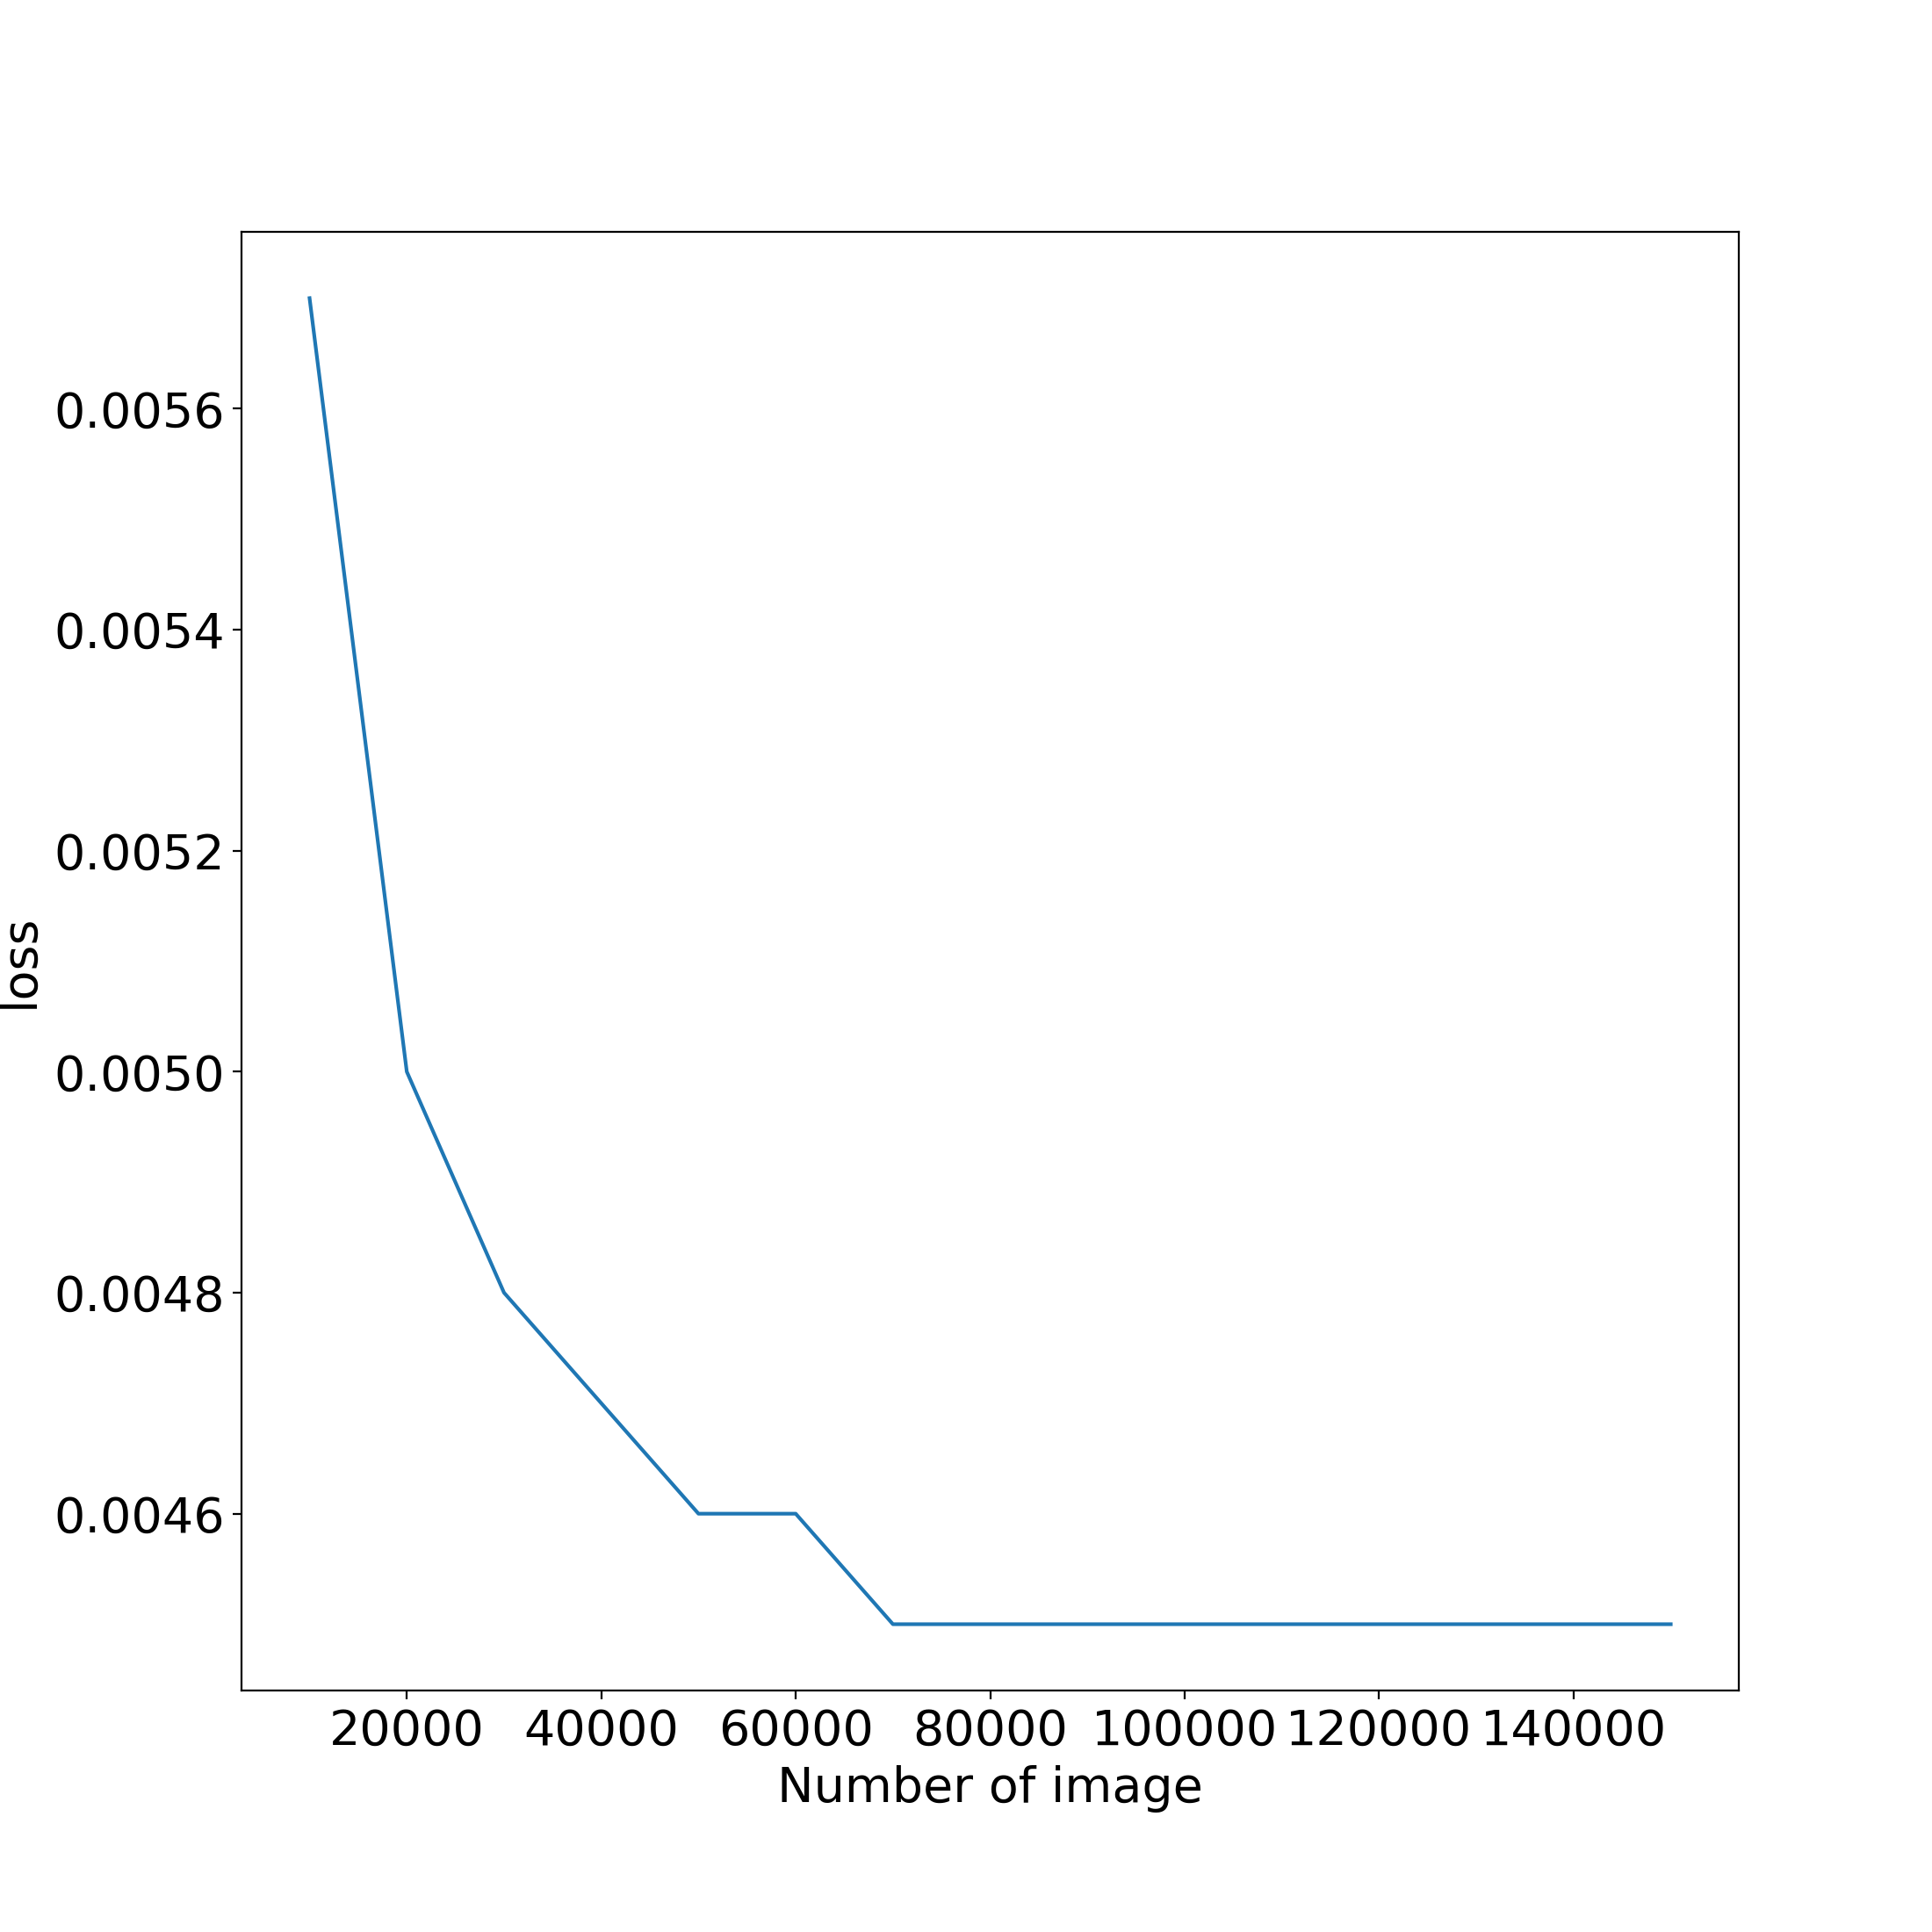
\includegraphics[width=8cm]{contents/evolution of training loss.png}
        \caption{Evolution of training loss}
        \label{Evolution of training loss}
    \end{center}
\end{figure}
\subsection{The choice of parameters}
In this section we will discuss the choice of the parameter in the network architecture and the choice of hyper parameters based on the training time, prediction results, which is calculated by PSNR formula, to find the best parameters.

First, we try to analyse the impact of channels of conv2d for the training time and the denoising effect of our network architecture, which is shown in Fig.2:
\begin{figure}[h]
    \begin{center}
        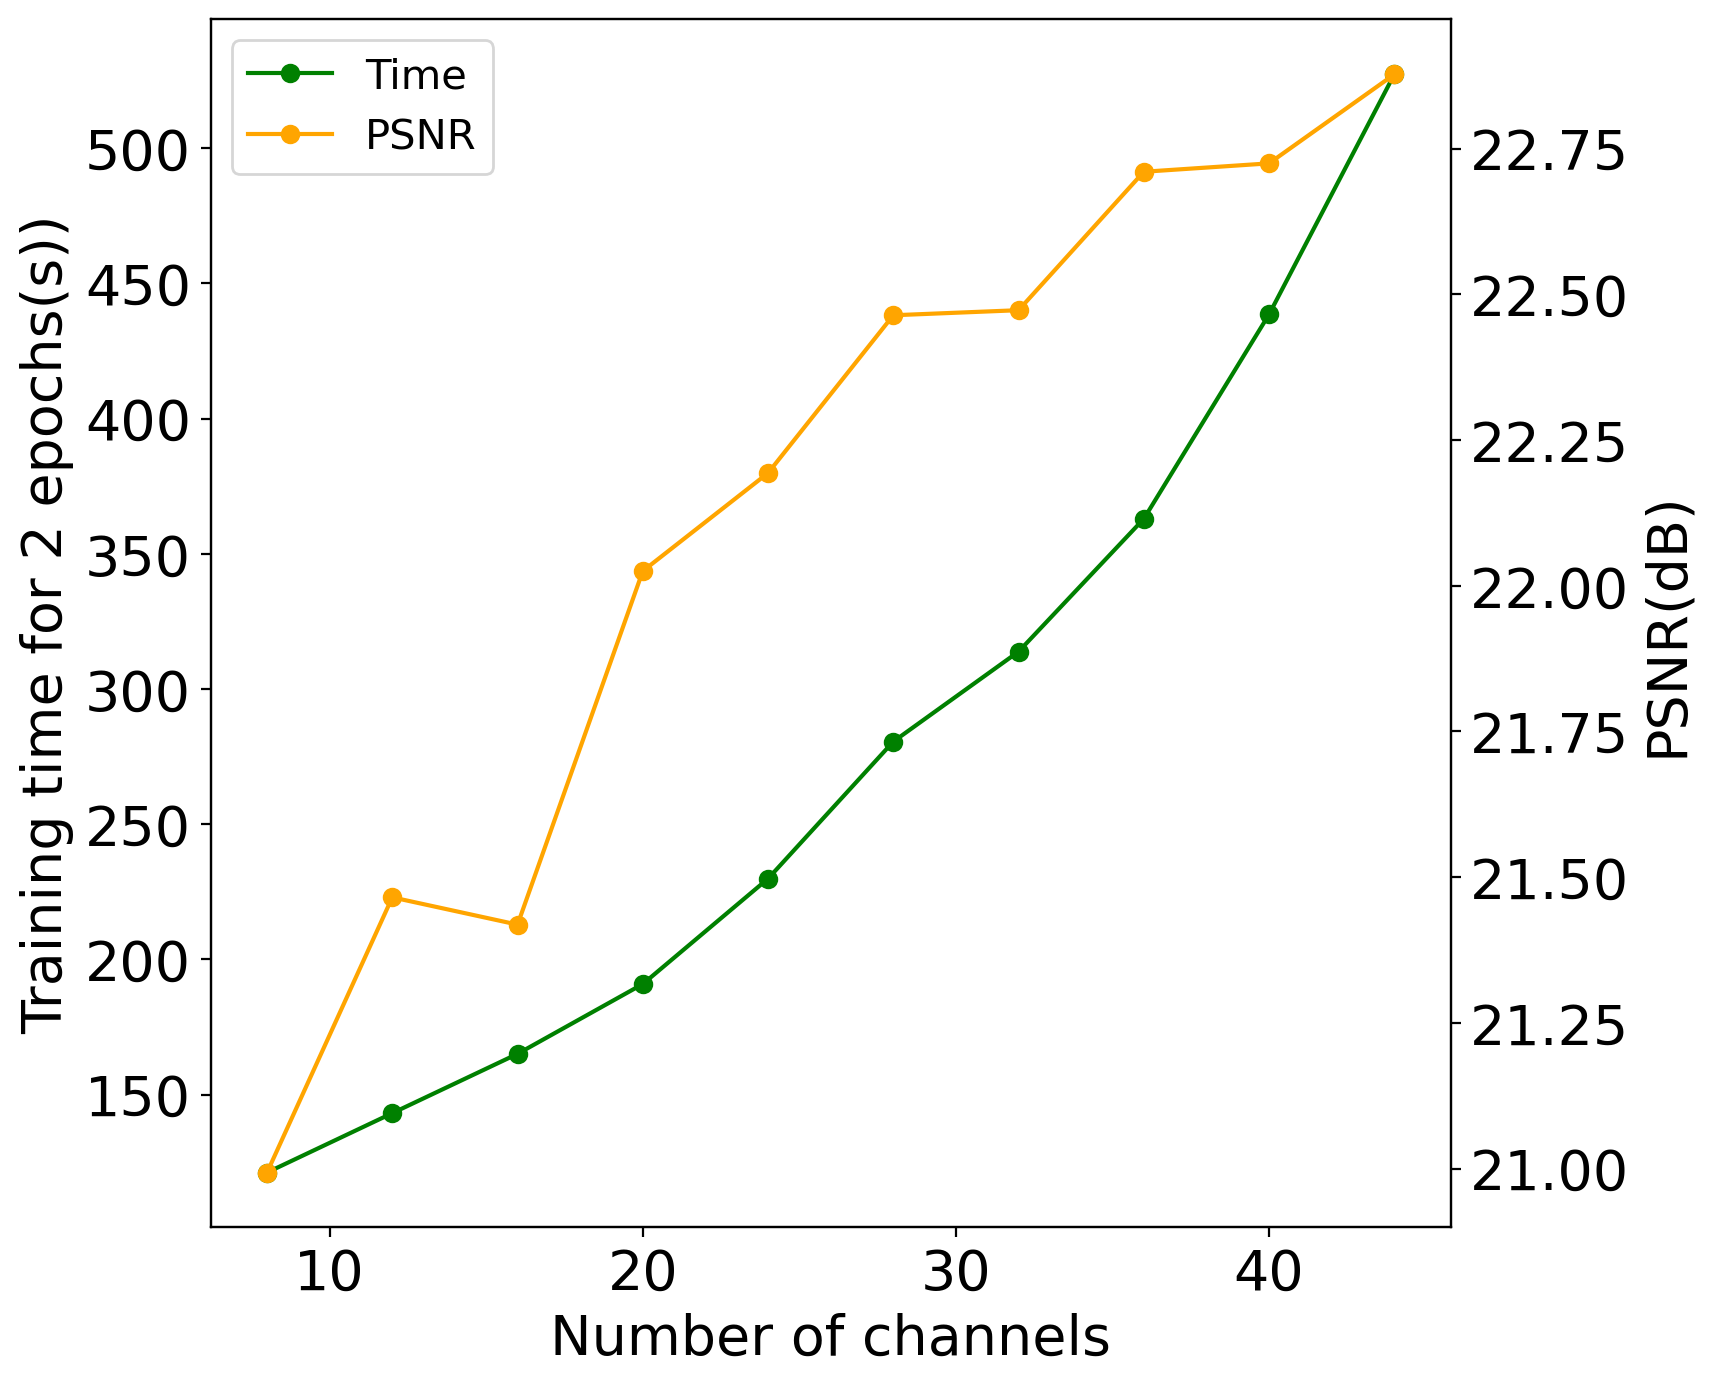
\includegraphics[width=7cm]{contents/channels.png}
        \caption{Impact of channels}
        \label{Impact of channels}
    \end{center}
\end{figure}

As we can see, with the increasing of the number of channels, the PSNR value is increasing, but at the same time, the training time is also increase, since the requirement for the training time of 1 epoch is below 5 minutes, we will use 44 channels for each convolutional layer.
\subsection{The choice of hyper parameters}
In this section, we will discuss the choice of learning rate and mini-batch size for our structure.

Firstly, we set different learning rate to find out the best one. Since if the learning rate is too small, it will take several epochs to get convergence, which is too time-consuming, we just consider the learning rate from 0.1 to 7, try to find the best one, the result is shown in Fig.3
\begin{figure}[h]
    \begin{center}
        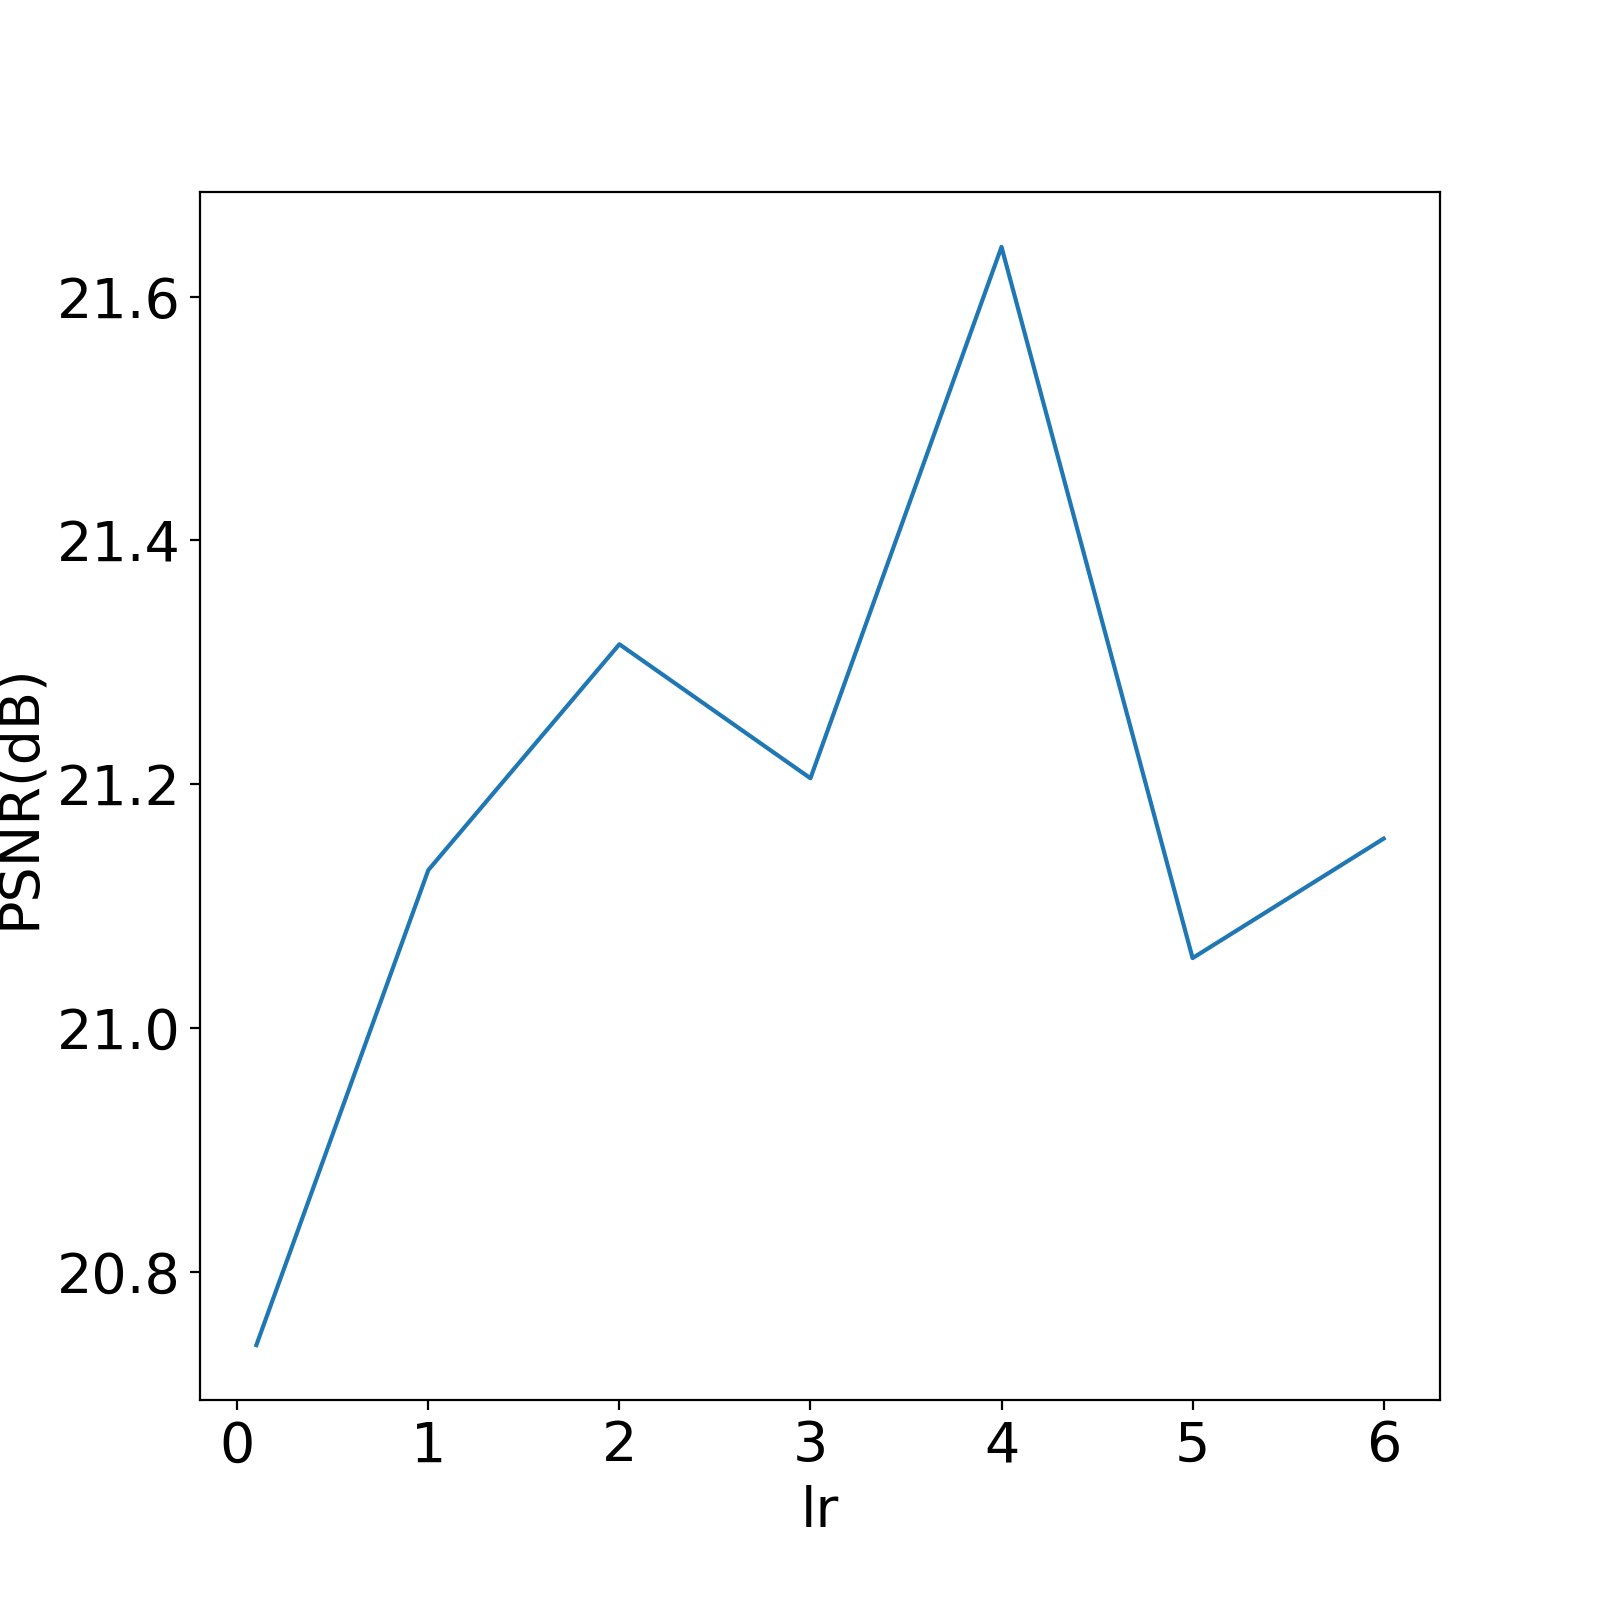
\includegraphics[width=8cm]{contents/lr.png}
        \caption{Impact of learning rate}
        \label{Impact of learning rate}
    \end{center}
\end{figure}
As we can see, the best learning rate is 4, so we choose it as our final choice.

Secondly, we consider the impact of mini-batch size for the denoising effect, which is shown in Fig.4.
\begin{figure}[h]
    \begin{center}
        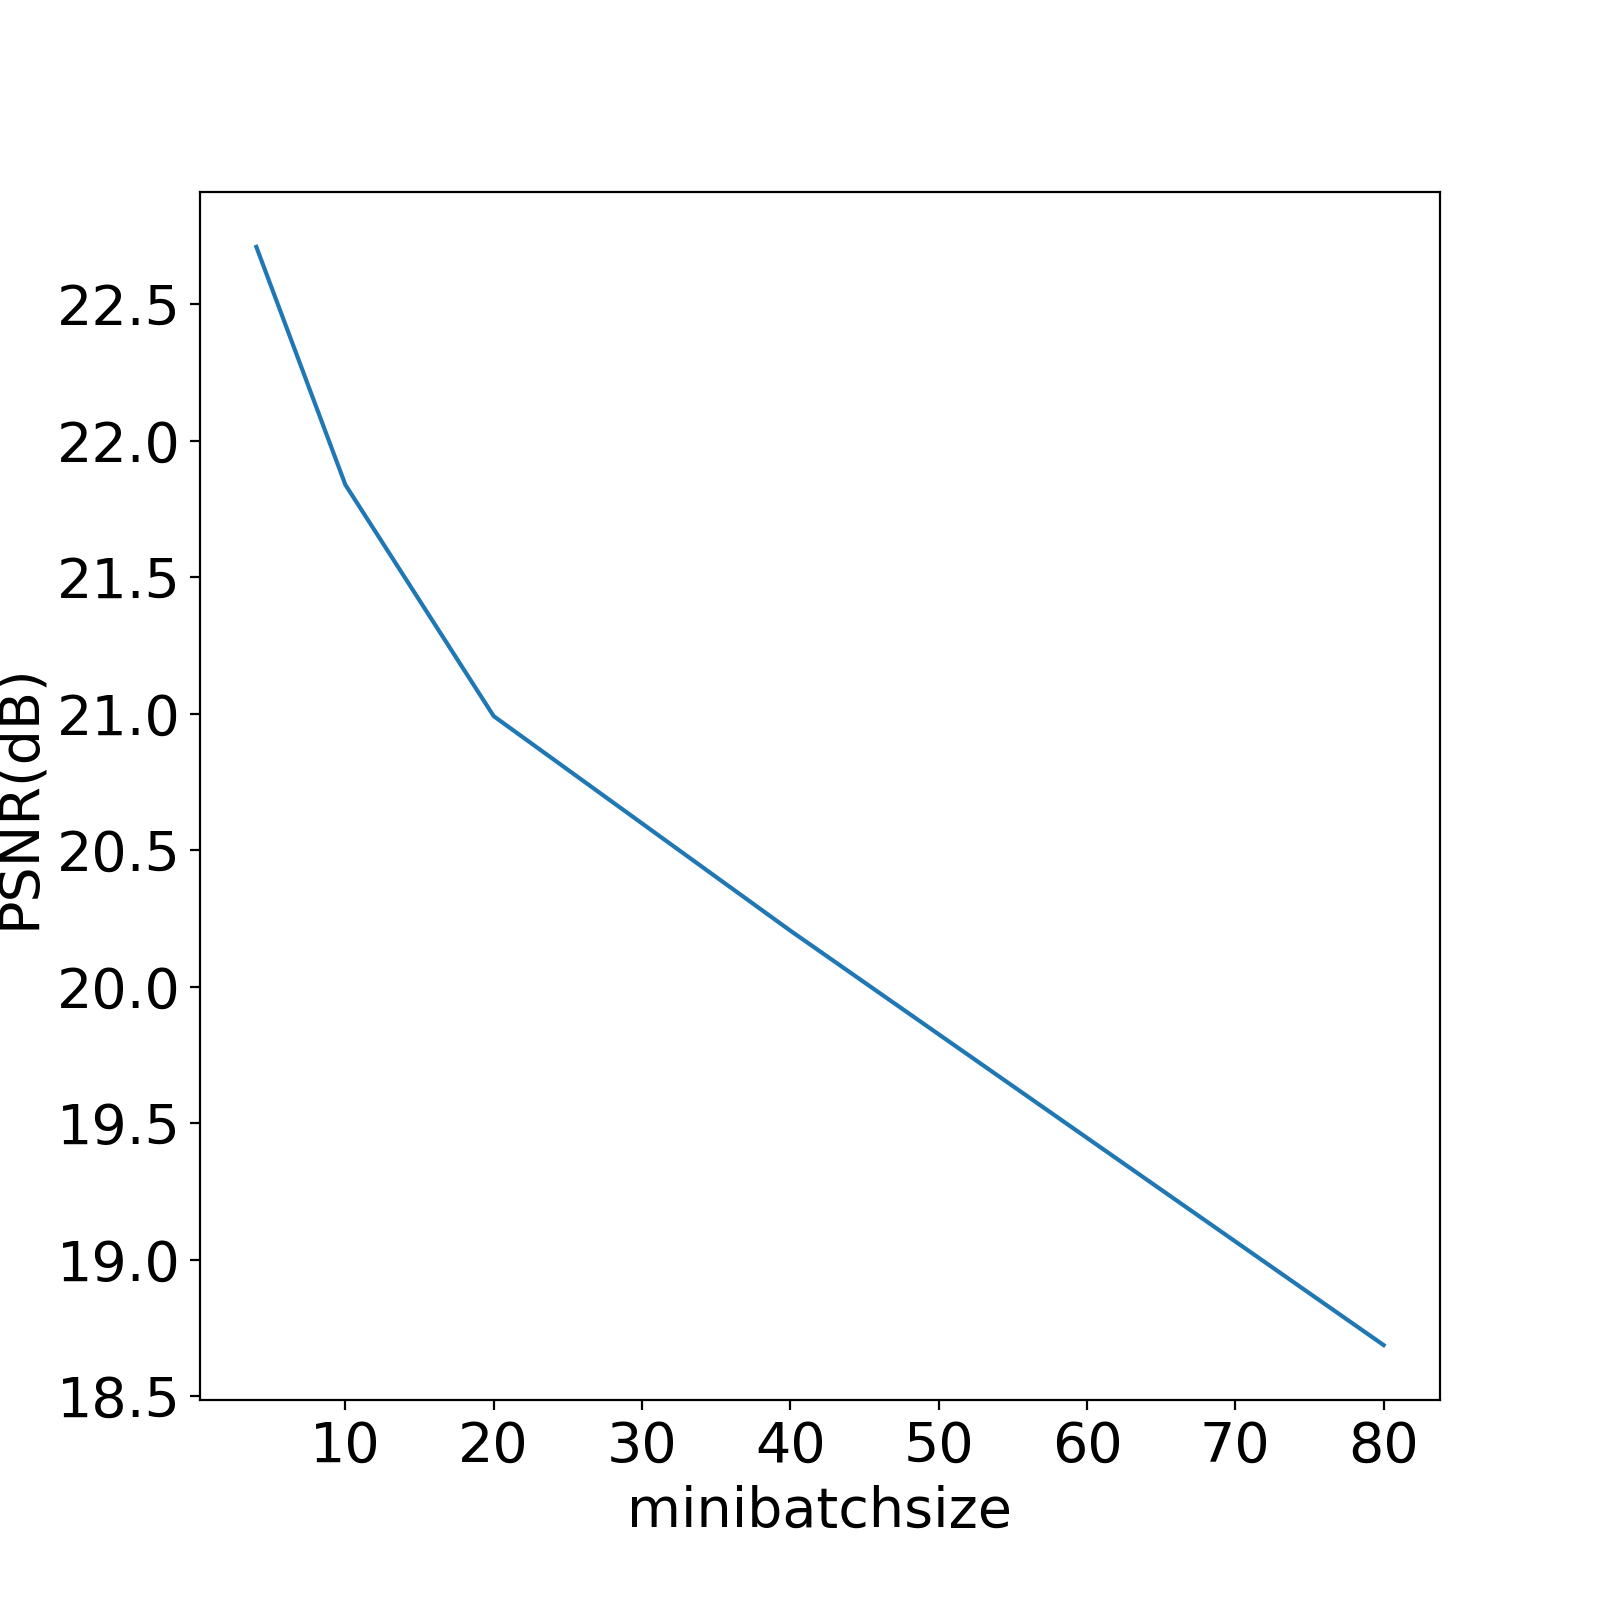
\includegraphics[width=9cm]{contents/minibatch.png}
        \caption{Impact of mini-batch size}
        \label{Impact of mini-batch size}
    \end{center}
\end{figure}
As we can see, with the increasing of the mini-batch size, the PSNR in decreasing, so we choose 4 as our final mini-batch size, which is the same as in the paper\cite{n2n}

Based on our best model architecture as well as the best hyperparameters, the average PSNR for the validation dataset is 22.81dB. Several denoised examples are also shown in Fig.5: 
\begin{figure}[h]
    \begin{center}
        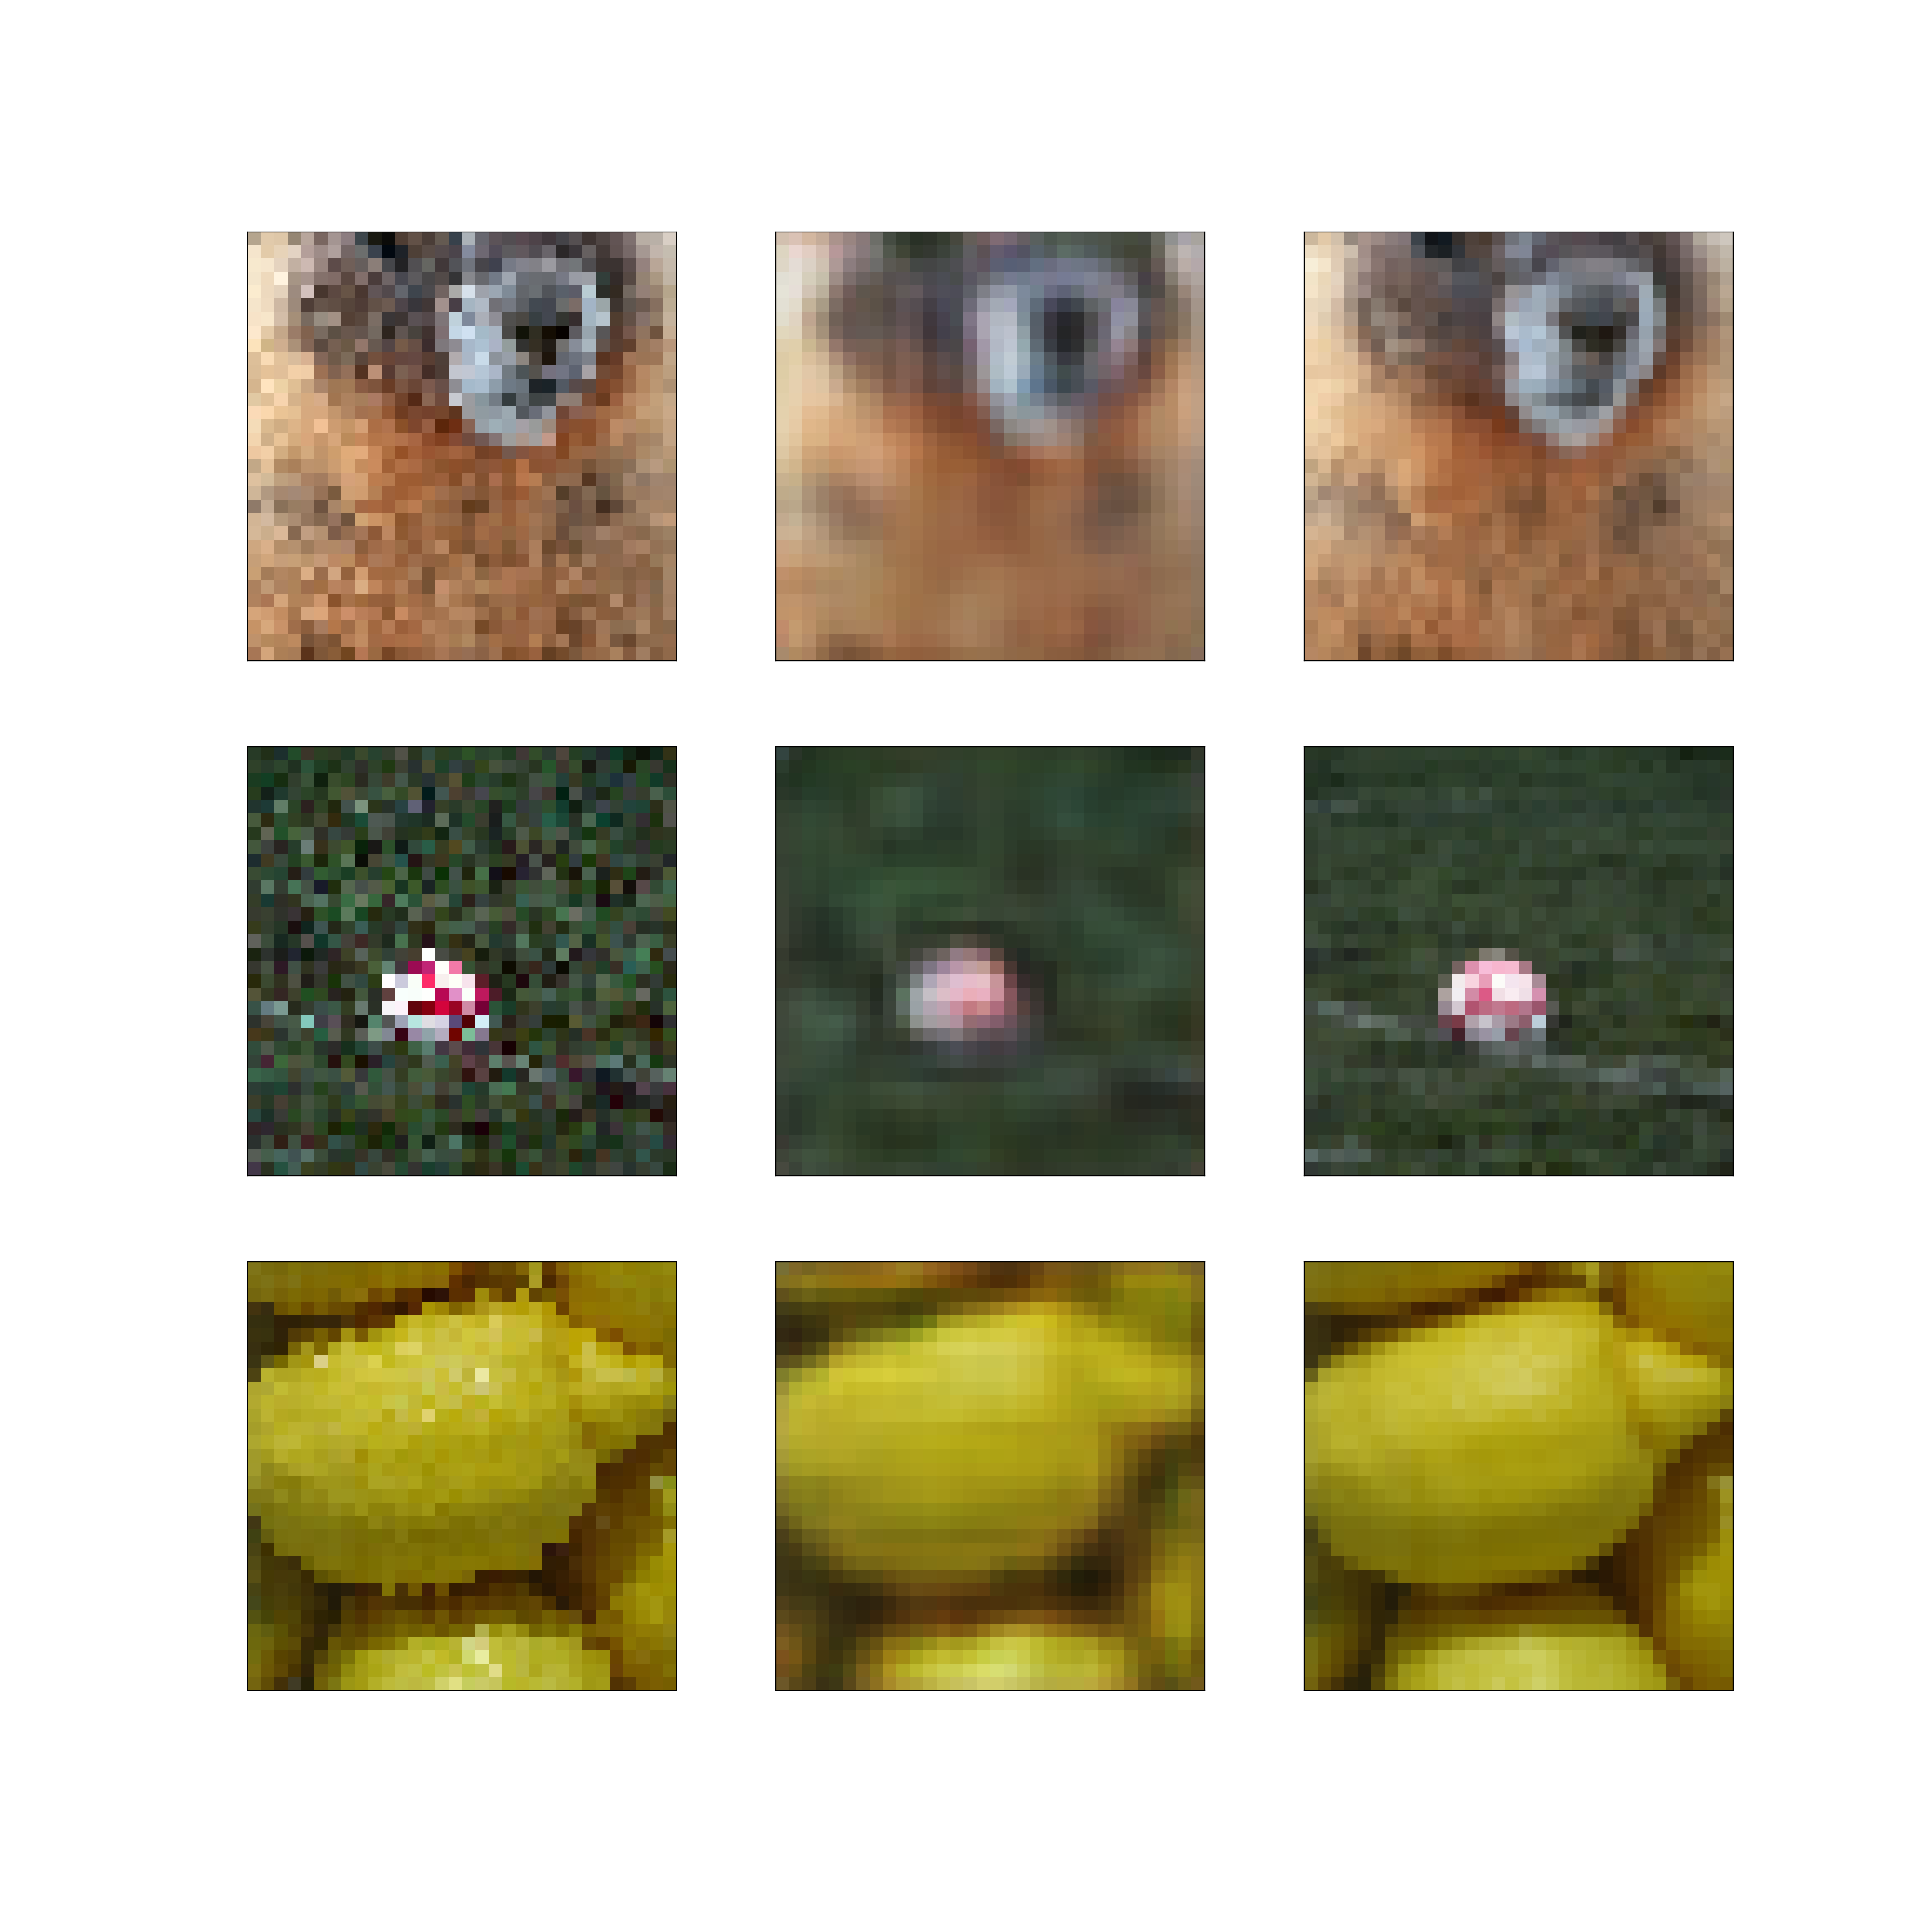
\includegraphics[width=9cm]{contents/comparison.png}
        \caption{Comparison between the validation target and prediction.The samples in the left column are the validation input samples, the samples in the middle column are our prediction results, the samples in the right column are the validation targets. The psnr of each row is 25.62dB, 24.77dB and 26.32dB.}
        \label{Comparison between the validation target and prediction}
    \end{center}
\end{figure}

